% !TeX encoding = UTF-8
% !TeX spellcheck = en_GB

%%% Add [final] option to the report class to switch between draft and final version of the report
%%% Use [narrowmargin] to enable narrow margins - this may impair readability.
%\documentclass[a4paper,12pt,draft]{include/intocpsreport}   %Or
\documentclass[a4paper,12pt,final]{include/intocpsassociation}   %Or
% intocpslargereport if chapters are required.
%
%
%
\usepackage[T1]{fontenc}
\usepackage[utf8]{inputenc}
\usepackage{longtable}
\usepackage{tikz-uml}
\usepackage{framed}
\usepackage{subcaption}
\usepackage[hyphenbreaks]{breakurl}
\usepackage{color}
\usepackage{amsmath}
\usepackage{courier}
\usepackage{xspace}
\usepackage{cleveref}
\usepackage{subcaption}
\usepackage{textcomp} % Used for 20-sim section \textrightarrow
%\usepackage{showframe}
\usepackage[section]{placeins}
\usepackage{listings}
\usepackage{glossaries}

%% Define listing environment for XML
\definecolor{gray}{rgb}{0.4,0.4,0.4}
\definecolor{darkblue}{rgb}{0.0,0.0,0.6}
\definecolor{cyan}{rgb}{0.0,0.6,0.6}

\lstset{
  basicstyle=\footnotesize\ttfamily,
  columns=fullflexible,
  showstringspaces=false,
  commentstyle=\color{gray}\upshape
}

\lstdefinelanguage{XML}
{
  morestring=[b]",
  morestring=[s]{>}{<},
  morecomment=[s]{<?}{?>},
  stringstyle=\color{black},
  identifierstyle=\color{darkblue},
  keywordstyle=\color{cyan},
  morekeywords={xmlns,version,type}% list your attributes here
}


\lstnewenvironment{xml}[1][]{\lstset{  language=XML,
  morekeywords={encoding, xs:schema,xs:element,xs:complexType,xs:sequence,xs:attribute}}\lstset{#1}}
{}

%% end listing environment for XML
%
%
%
\def\draftnote#1{\noindent\smallskip\framebox{\begin{minipage}{0.95\columnwidth}\color{red}#1\end{minipage}}\smallskip\par}
\newenvironment{draftnoteenv}{\noindent\smallskip\begin{framed}\begin{minipage}{0.95\columnwidth}\color{red}}{\end{minipage}\end{framed}\smallskip\par}
\newenvironment{assumption}{\noindent\smallskip\color{blue}\begin{framed}\begin{minipage}{0.95\columnwidth}}{\end{minipage}\end{framed}\smallskip\par}
%
%
%
\newcommand{\revisit}[1]{\textcolor{red}{\pmb{[[[}\@ #1\@ \pmb{]]]}}}
%
%
\reporttitle{INTO-CPS External Data Broker FMU\\\vspace{1em} (RabbitMQ FMU)}
\shortreporttitle{INTO-CPS EDB FMU}  %To use if report title is too long for header
%
%
%
%%% Set document release class as appropriate
%%% e.g. Public, Restricted, Programme Participant
\reportstatus{Public Draft}
%
%
%
%%% If document is a deliverable, this flag should be commented out
%%% e.g. %\technotetrue
%%% If report is a technical report, leave uncommented
%%% e.g. \technotetrue
\technotetrue % Comment out as appropriate
%
%
%
\submissiondate{}
\contributors{
Kenneth Lausdahl, AU \\
Casper Thule, AU
}
%
%
%
\editors{
  Casper Thule, AU \\
  Kenneth Lausdahl, Mj\olner Informatics A/S
}
%
%
%
%\reviewers{Ken Pierce, UNEW\\
%Kangfeng Ye, UY\\
%Luis Diogo Couto, UTRC}
%
%
%
%% Version details
% #1: version
% #2: date
% #3: author
% #4: description
\addversion{0.01}{January 13, 2019}{Casper Thule}{Initial Version.}

%
%
\begin{document}
\maketitle
%
%
%
%%%% Document abstract page %%%%
\section*{Abstract}
\label{sec:abstract}
%
TBD
%
\newpage
%
%%%% Document table of contents page %%%%
\tableofcontents
\newpage
%
%
%
%%%% Document Content %%%%
%% \chapter{Chapter Title} %% if intocpslargereport is in use
%\begin{assumption}
%
%
%
\section{Introduction}\label{sec:intro}
EDB is short for External Data Broker and EDB FMU is an FMU that brings external
data into an FMI context. The implementation of EDB FMU described in this
publication is based on RabbitMQ. However, this is just one way to implement an
EDB FMU. Several of the constructs described in this publication are general and
can be used with other message-oriented or data streaming middleware. For this
reason, both EDB FMU and RabbitMQ FMU will be used throughout this document,
where EDB FMU is generally applicable functionality, whereas RabbitMQ FMU is an
implementation of EDB FMU specific to RabbitMQ. Thus, one could take the
existing source code of RabbitMQ FMU and fit it to another middleware than
RabbitMQ while still reusing most of the source code.
Note, that this document assumes general knowledge of
the Functional Mock-up Interface (FMI)~\cite{FMIStandard2.1}.

An overall approach to using an EDB FMU in a digital twin context is depicted
in~\cref{fig:interfacing_overview}, where the content within the \textit{System Specific} frame will vary based on the system
providing the data. The Log-Translator entity translates the
system-specific log messages to digital twin compatible messages and publishes
them to a Data Middleware Node (i.e. a RabbitMQ Node). The EDB FMU is configured
via its static description to
receives messages from the Data Middleware Node. The message content is then
parsed and published via regular FMI outputs.

\begin{figure}[htb]
  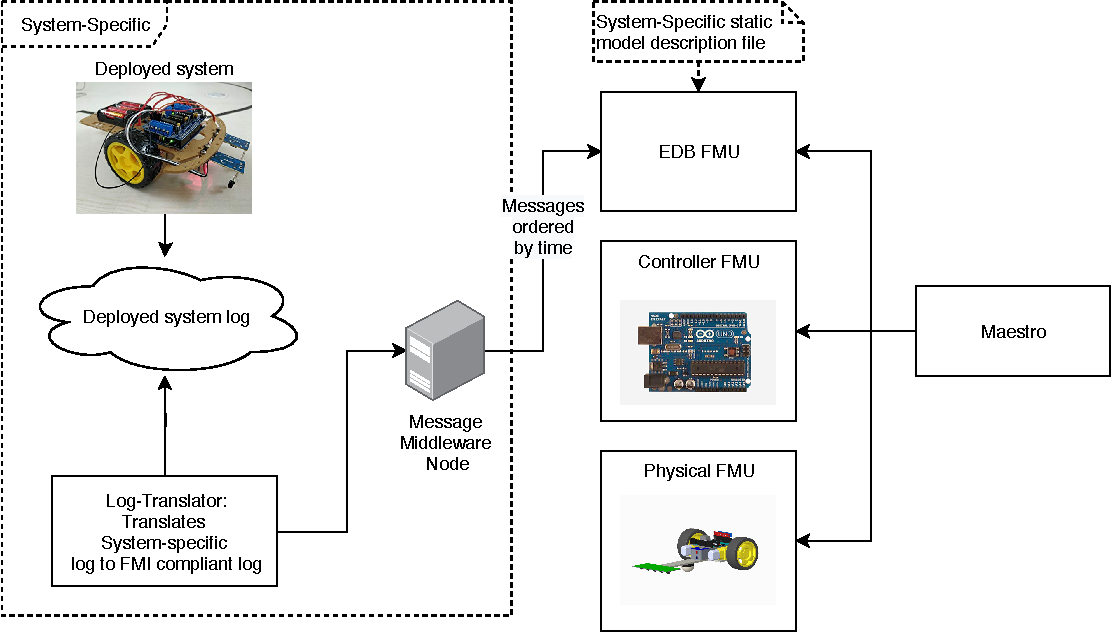
\includegraphics[width=\textwidth]{figures/overview.pdf}
  \caption{Interfacing Overview}
 \label{fig:interfacing_overview}
\end{figure}

This approach generalises the FMI enabling entity, the EDB FMU, such that
it can be used for different kinds of systems with different kinds of logging
facilities. The motivation behind this approach is that tools of the INTO-CPS Association
should be generally applicable.

The following chapters describes the following in order:
\begin{description}
  \item[Time Handling] How system-time and simulation time is mapped and put in
    an FMI simulation context.
  \item[Data Handling] How message content and the state of EDB FMU are
    coordinated.
  \item[Configuration] How to configure an EDB/RabbitMQ FMU via the ModelDescription File
  \item[Example - Single Water Tank RabbitMQ] This example demonstrates how RabbitMQ FMU
    acts as an External Data Broker in context of a Single Water Tank Digital Twin. It focuses solely on this part and does not
    contain a deployed system.

    \item[Example - Line Following Robot] IN PROGRESS - This example demonstrates transmission
    of data from a deployed line following robot. The data is made available in
    the FMI co-simulation via RabbitMQ FMU. Thus, this is a example with
    both a deployed system, its digital twin and the RabbitMQ FMU.
  \item[Future Work] Describes some ideas for future work.
\end{description}


%%% Local Variables:
%%% mode: latex
%%% TeX-master: "../rabbitmq-fmu"
%%% End:

\newpage
\section{Time Handling}\label{sec:time_handling}
This section concerns the digital twin and how data time is handled with
relation to FMI.
The description below is accompanied by \cref{fig:time-handling_simulation-view}.

\begin{figure}[!htb]
  \centering
  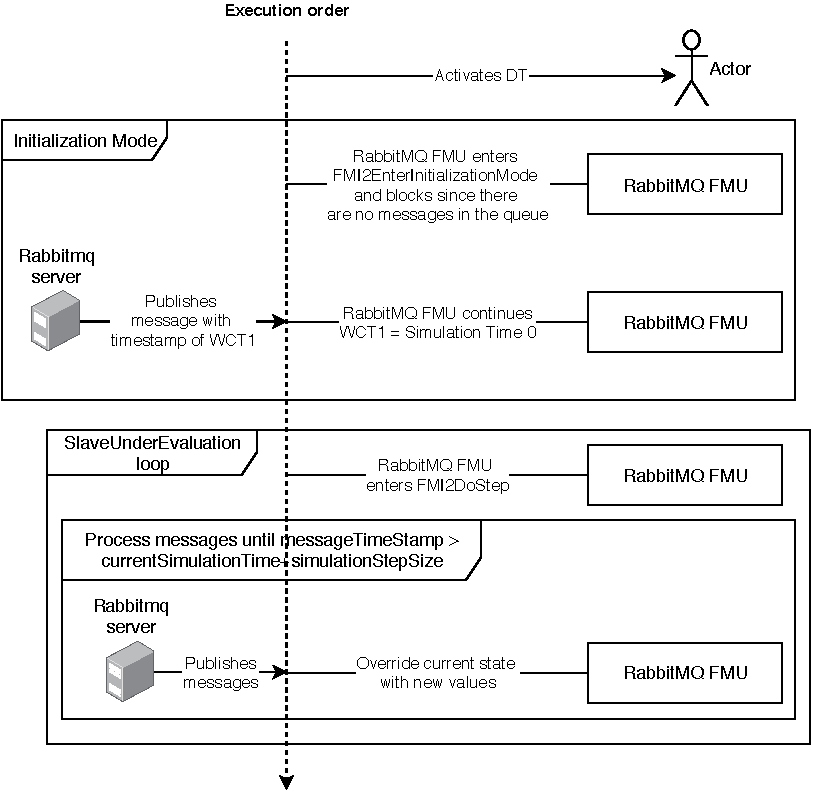
\includegraphics[width=\textwidth]{figures/timehandling.pdf}
  \caption{Time Handling in Simulation View}
  \label{fig:time-handling_simulation-view}
\end{figure}

Invoking the function \texttt{fmi2EnterInitializationMode} on EDB FMU causes it to
block until a message is available.\\
The time stamp of the first message ($WCT1$) received defines $simulationTime0$ and EDB
FMU continues. Thus $WCT1 = simulationTime0$ and a mapping between WCT and simulation time is
establishedcreated. Thus, any subsequent timestamps has $WCT1$ subtracted in order to map
them to $simulationTime$.\\
This also implies that any message with a time stamp of $WCT 0 < WCT1$ are ignored.

Invoking the function \texttt{fmi2DoStep} on EDB FMU causes it to process
messages and keep executing until there is a message with a time stamp defined by
$message\-TimeStamp\-InSimulationTime >= currentSimulationTime +
simulationStepSize$. Such a message is stored in order to use it for the
subsequent \texttt{fmi2DoStep} operation.

%%% Local Variables:
%%% mode: latex
%%% TeX-master: "../rabbitmq-fmu"
%%% End:

\newpage
\section{Data Handling}\label{sec:data_handling}
The data handling occurring within \texttt{fmi2DoStep} of EDB FMU is described
below.
All values of messages with time stamps (converted to simulation time) within the
time interval $]currentSimulationTime,currentSimulationTime + simulationStepSize]$
overrides the current state of values in the received order, thus using
zero-order hold. This depends on the Data Middleware Node providing the data
order by time, as mentioned in \cref{sec:intro}.

An example is given in \cref{fig:data-handling-dostep}.
First, \texttt{message x} is received and overwrites the value of \texttt{a} in the EDB FMU state.\\
Afterwards, \texttt{message y} is received and overwrites the value of \texttt{b} in
the EDB FMU state.\\
Lastly, \texttt{message z} is received and overwrites the value of
\texttt{a} in the EDB FMU state. \\
The example above implies that the value of \texttt{a} in \texttt{message x}  is never
outputted from the EDB FMU, since it has been overwritten by the value of
\texttt{a} in \texttt{message z} within the same \texttt{fmi2DoStep} execution.

\begin{figure}[htb]
  \centering
  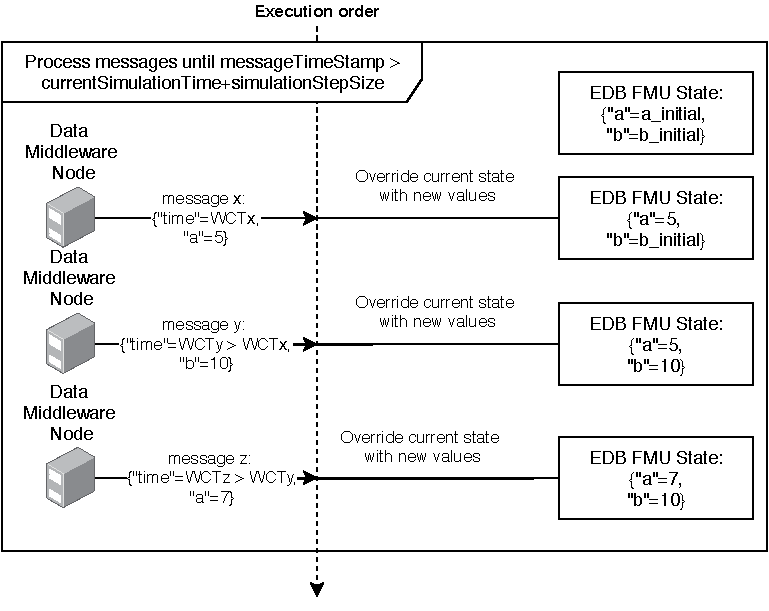
\includegraphics[width=\textwidth]{figures/datahandling.pdf}
  \caption{Data Handling in \texttt{fmi2DoStep}}
  \label{fig:data-handling-dostep}
\end{figure}

%%% Local Variables:
%%% mode: latex
%%% TeX-master: "../rabbitmq-fmu"
%%% End:

\clearpage
%
%
%
%
%%%% Bibliography %%%%
\bibliographystyle{alpha}
\bibliography{bibliography}
\label{ch:bib} %label to refer to
%
%
%
\clearpage
%
%
%
\appendix
\section{List of Acronyms}\label{appendix:acronyms}
\begin{longtable}{ll}
XML	&Extensible Markup Language\\
\end{longtable}

\clearpage
%
%
%
\end{document}

%%% Local Variables:
%%% mode: latex
%%% TeX-master: t
%%% End:
